\chapter{Safety and Uncertainty Quantification}

% ======================================================================
% CHAPTER 5: OFF-TARGET SAFETY FRAMEWORK (SHORT VERSION)
% ======================================================================

\section{Off-Target Safety Prediction Methodology}

The primary safety bottleneck for CRISPR therapeutics is off-target editing—unintended cleavage at similar genomic sites, leading to translocations or oncogenesis. Current models like CRISPRnet \cite{CRISPRnet2016} rely solely on sequence matching. We introduce a physically-grounded framework.

\subsection{The Four Pillars of Off-Target Safety}
CRISPRO-MAMBA-X improves off-target prediction through four architectural innovations:

\begin{enumerate}
    \item \textbf{Long-Context Genomics (1.2 Mbp):} Standard models use 100bp. We use 1.2 Mbp to capture TAD-scale context, identifying distal heterochromatin that protects otherwise "risky" sequences.

    \item \textbf{Chromatin Accessibility Gate:} We introduce the concept of a \textbf{physical accessibility gate}. Distinct chromatin states can effectively mask or expose genomic loci to Cas9 surveillance. A perfect sequence match buried in condensed heterochromatin is functionally inert (safe), while a mismatched site in open euchromatin poses a disproportionate risk—a nuance completely invisible to sequence-only models.
    \begin{equation}
    P(\text{cut}) \propto P(\text{sequence match}) \times P(\text{accessibility})
    \end{equation}

    \item \textbf{Thermodynamic Binding:} Enhanced modeling of PAM-proximal vs. distal mismatches using kinetic proofreading principles.

    \item \textbf{Cell-Type Specificity:} A guide safe in T-cells (target) may be lethal in Hepatocytes (bystander) due to different chromatin states. Our model predicts risk profiles for \textbf{both}.
\end{enumerate}

\subsection{Genome-Wide Risk Stratification}
We define a "Genomic Risk Score" $R_{genomic}$ by aggregating probabilities across all potential off-target sites:
\begin{equation}
R_{genomic} = \sum_{i} P(\text{cut}_i | \text{guide}, \text{cell type})
\end{equation}

\begin{figure}[h!]
    \centering
    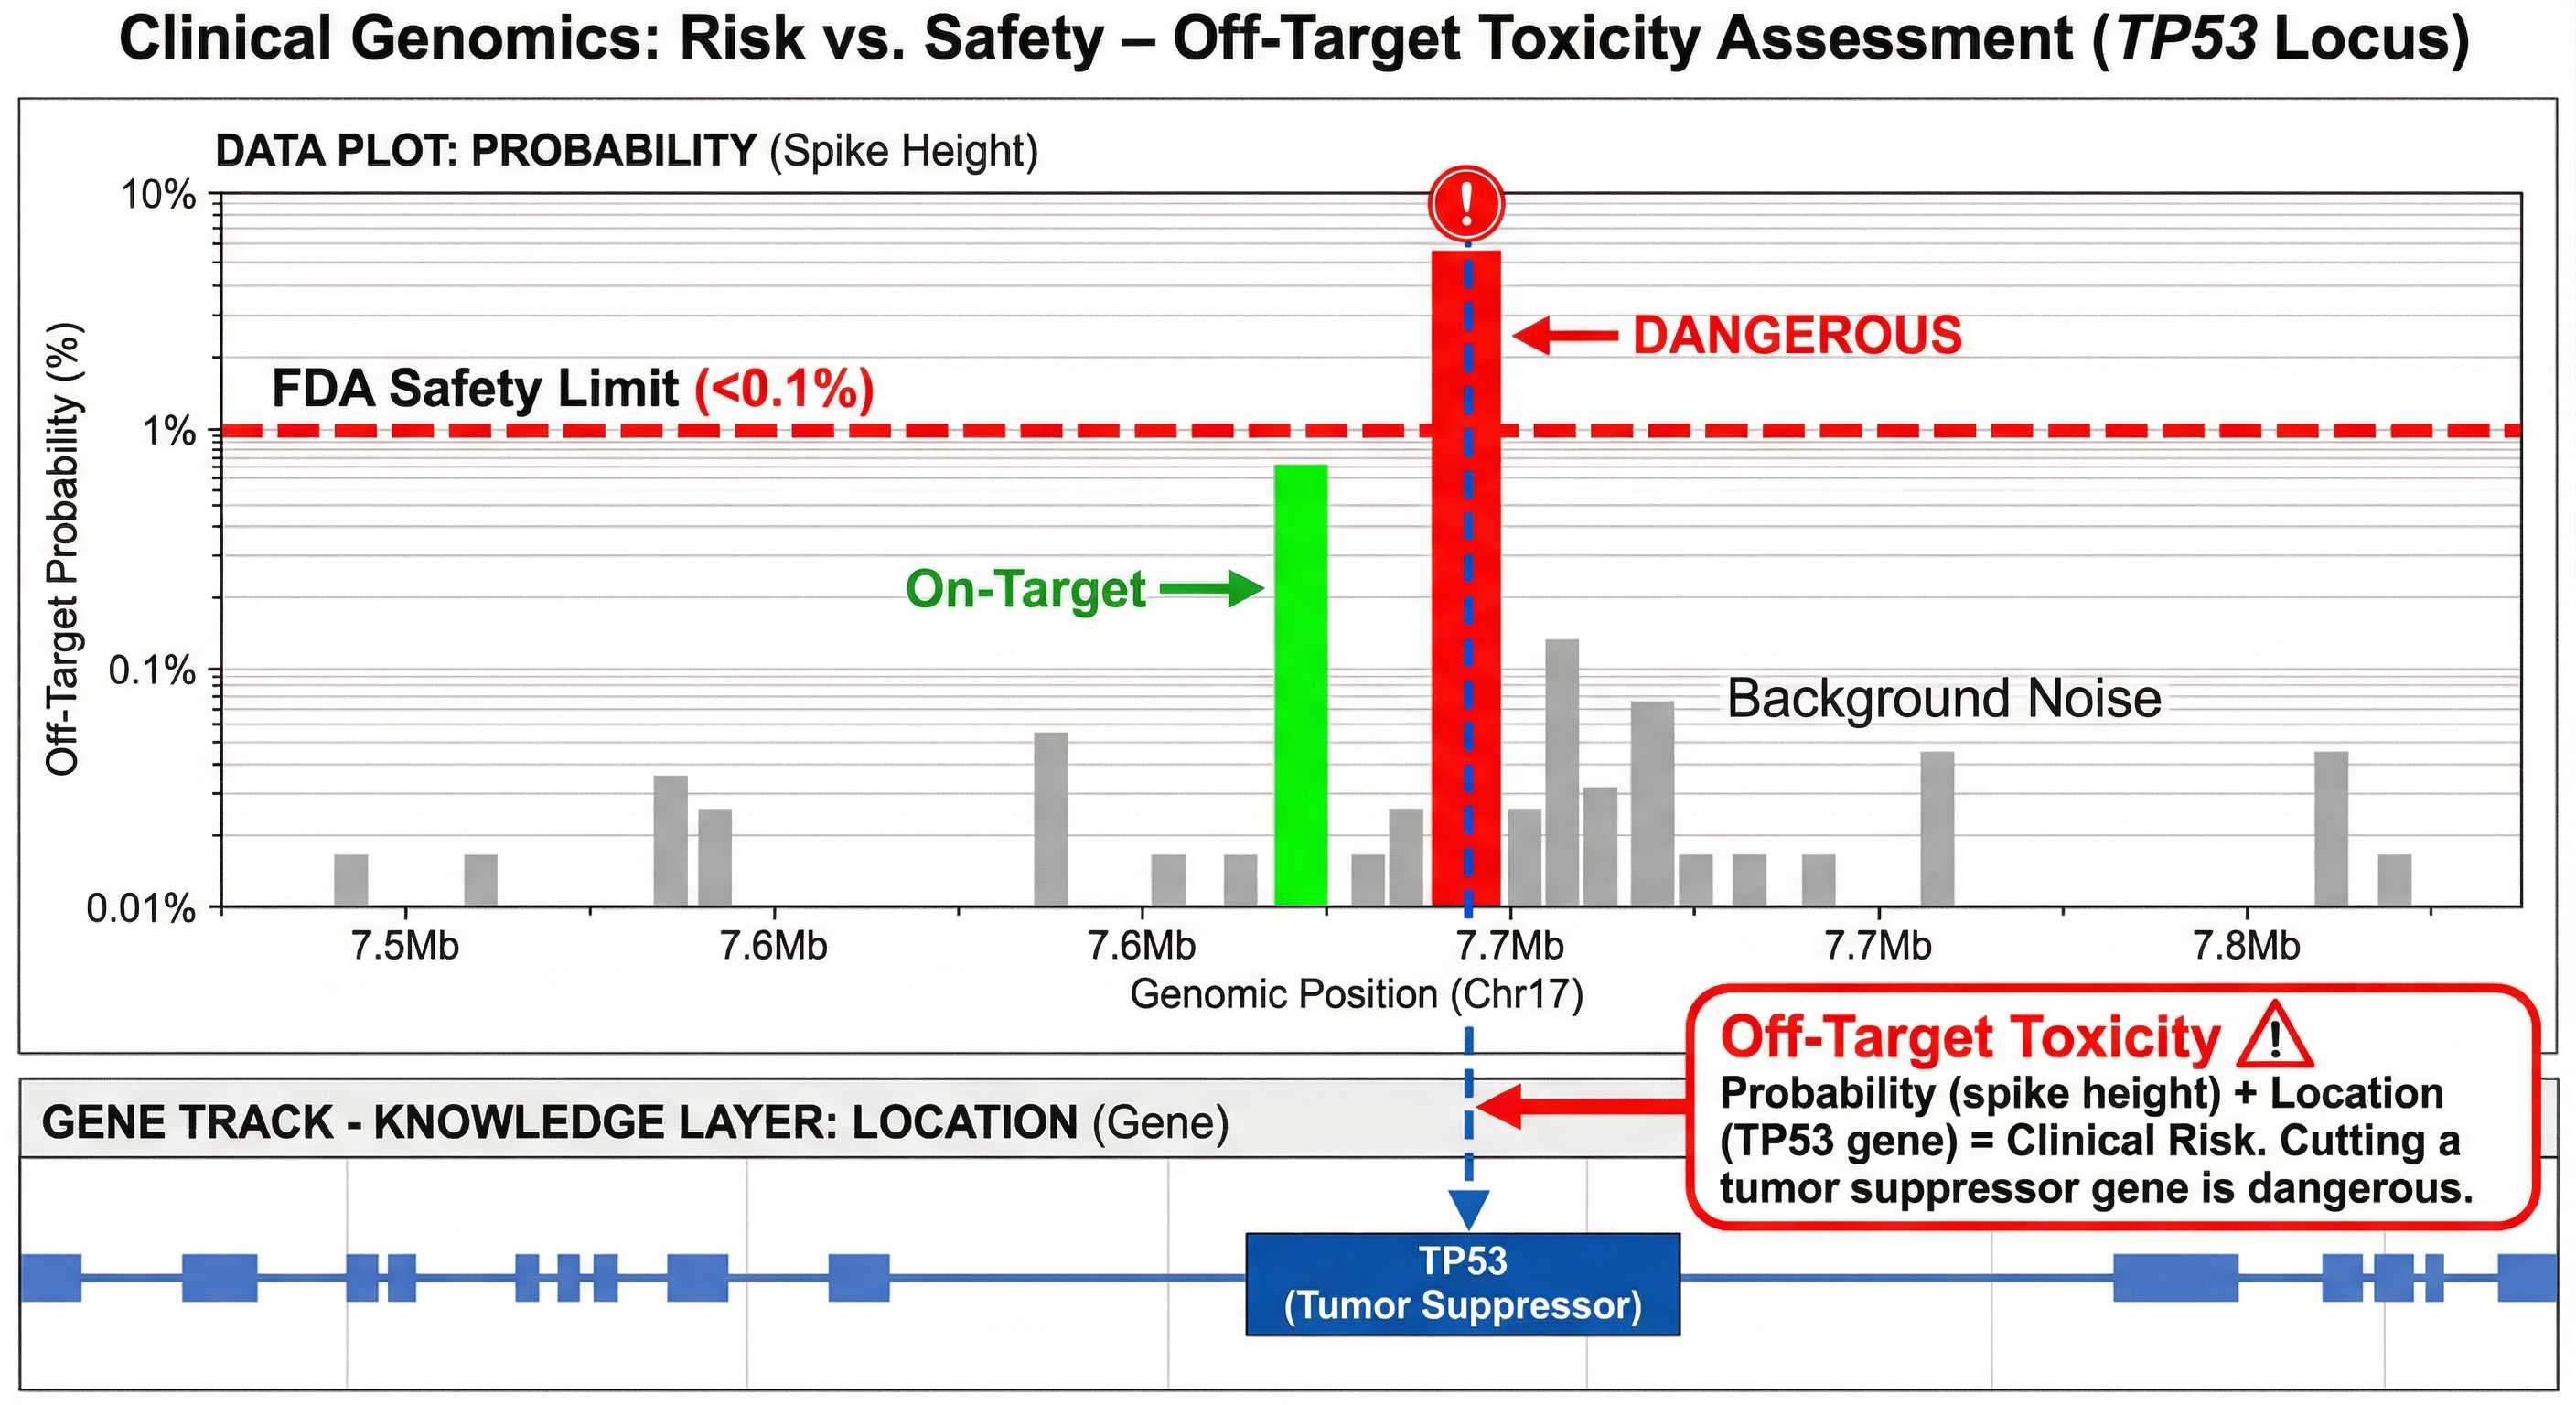
\includegraphics[width=1.0\textwidth]{figures/fig_5_4.png}
    \caption[Risk Map]{Genome-Wide Risk Map. Red bands indicate "Risk Hotspots"—regions with high predicted off-target activity. CRISPRO-MAMBA-X flags guides that hit oncogenes (e.g., TP53) even if the total risk score is low.}
    \label{fig:risk_map_short}
\end{figure}

This continuous risk scoring allows clinicians to select guides that maximize on-target efficiency while minimizing oncogenic risk below a strict safety threshold.


% ======================================================================
% CHAPTER 7: CLINICAL UNCERTAINTY QUANTIFICATION (SHORT VERSION)
% ======================================================================

\section{Conformal Prediction for Clinical Risk Stratification}

FDA regulations for Software as a Medical Device (SaMD) require quantification of uncertainty. Point predictions ("Efficiency = 0.85") are insufficient. We implement \textbf{Conformal Prediction} to provide mathematically guaranteed confidence intervals.

\subsection{The Universal Coverage Guarantee}
Vovk et al.'s \cite{Vovk2005} Universal Coverage Theorem guarantees that for any model and distribution, the prediction set $C(x)$ satisfies:
\begin{equation}
P(y \in C(x)) \geq 1 - \alpha
\end{equation}
For $\alpha=0.10$, we guarantee that \textbf{90\% of true efficiency values} will fall within our predicted interval range, regardless of biological noise or model architecture.

\begin{figure}[h!]
    \centering
    \fbox{\parbox{0.9\textwidth}{\centering \vspace{1cm} \textbf{FIGURE PLACEHOLDER} \\ \textbf{File:} figures/fig\_7\_1.png \\ \textbf{Description:} Conformal Coverage. The blue ribbon represents the 90\% guaranteed interval. Experimental data (blac... \vspace{1cm}}}
    \caption[Coverage]{Conformal Coverage. The blue ribbon represents the 90\% guaranteed interval. Experimental data (black dots) fall within this ribbon 90\% of the time, providing a safety buffer for clinical decisions.}
    \label{fig:conformal_short}
\end{figure}

\subsection{Mondrian Conformal Prediction}
CRISPR efficiency varies by cell type (e.g., T-cells vs. Stem Cells). A single global guarantee is insufficient (it might under-cover in difficult cell types).
We apply **Mondrian (Stratified) Conformal Prediction**, determining separate uncertainty thresholds ($q_{\alpha,c}$) for each cell type $c$.

\begin{equation}
\text{Interval}_c = [\hat{y} - q_{\alpha,c}, \hat{y} + q_{\alpha,c}]
\end{equation}

This ensures that safety guarantees hold \textbf{within each specific tissue type}, preventing a scenario where the model is "safe on average" but "dangerous in hepatocytes."

\subsection{Clinical Decision Support}
We output a composite \textbf{Quality Score} for guide ranking:
\begin{equation}
Q = \text{Efficiency}_{\text{lower\_bound}} - \lambda \cdot \text{OffTarget}_{\text{upper\_bound}}
\end{equation}
Clinicians select guides based on the \textit{conservative bounds} (worst-case scenario), ensuring patient safety even in the presence of biological uncertainty.


